\section{Moteur de jeux combinatoires abstraits et algorithmes}


% présenter les principaux algorithmes utilisés comme moteur de jeu combinatoires absrtaits
%methode de monte carlo
%min max


% evaluer la complexité théorique en temps des algorithmes présentés.

Implémenter un algorithme pour jouer à des jeux combinatoires contre l'ordinateur est l'un des objectifs principaux du projet
Hex-Ta(c)tique, mais plusieurs questions naturelles ont alors vu le jour: quels sont les algorithmes qui permettent à un ordinateur
de jouer à un jeu combinatoire abstrait ? Quels sont leurs points forts et faibles ? Dans cette section, nous allons
présenter deux algorithmes principaux qui aident à répondre à ces questions: la recherche arborescente \emph{Monte-Carlo} (Monte-carlo Three Search) 
et l'algorithme du \emph{MinMax} avec élagage alpha-bêta:

\subsection{La recherche arborescente Monte-Carlo}

\paragraph{Présentation}
La recherche arborescente Monte-Carlo ou Monte-Carlo Tree Search (MCTS) est un algorithme de recherche heuristique.
Il est principalement utilisé dans le cadre de mise en place d'intelligence artificielle pour des jeux tels que le go, mais pas uniquement.
En effet, il peut aussi être utilisé pour les moteurs de jeux des échecs comme le moteur AlphaZero de Google qui est
l'un des leaders en termes d'intelligence de jeux aux échecs. Cet algorithme peut même être implémenté dans des jeux où le hasard 
apparaît par exemple au poker.

\paragraph{MCTS - Fonctionnement succinct}
MCTS est un algorithme qui explore l'arbre des possibles. La racine est la configuration initiale du jeu.
Chaque nœud est une configuration (une situation en jeu) et ses enfants sont les configurations suivantes. MCTS conserve en mémoire 
un arbre qui correspond aux nœuds déjà explorés. Une feuille de cet arbre est soit une configuration finale (donc un des joueurs a gagné),
soit un nœud dont aucun enfant n'a encore été exploré. Dans chaque nœud, on stocke deux nombres : le nombre de simulations gagnantes, 
et le nombre total de simulations. 

À chaque itération MCTS va chercher la feuille la plus prometteuse, comprendre la suite de coups qui possède la meilleure heuristique, 
et ensuite, depuis cette feuille, créer grâce aux règles du jeu, une nouvelle feuille au hasard dont le but est d'atteindre une configuration finale.
Dans le cas où on trouverait une configuration gagnante pour un joueur, on va incrémenter le nombre de simulations gagnantes, pour les nœuds
correspondant au joueur et dans les parents de la feuille que l'on vient de créer.
L'algorithme répète cette opération un certain nombre de fois avant de choisir un coup, ie: choisir le coup qui a le plus de simulations
gagnantes et le moins de simulations totales.

%exemple.\dots


\subsection{MinMax}

\subsubsection{Présentation}
L'algorithme MinMax, comme MCTS, est un algorithme décisionnel. Cependant, celui-ci s'applique sur des jeux à somme nulle: c'est-à-dire
un jeu où la somme des gains et des pertes de tous les joueurs est égale à 0. Ainsi, le gain de l'un constitue 
obligatoirement une perte pour l'autre. L'algorithme va utiliser cette propriété dans sa recherche pour trouver le meilleur coup possible.
En effet, l'ordinateur va passer en revue toutes les configurations possibles pour un nombre limité de coups (que l'on appellera profondeur), 
et leur assigner une valeur qui prend en compte les bénéfices pour le joueur et pour son adversaire. Le meilleur coup est alors celui qui 
minimise les pertes du joueur, tout en supposant que l'adversaire cherche au contraire à les maximiser (d'où le nom MinMax).

\subsubsection{MinMax - Fonctionnement succinct}
Comme le MCTS, le MinMax va explorer l'arbre des possibles où chaque nœud représente une configuration du jeu. 
L'algorithme va explorer toutes les possibilités et associer à chaque feuille une valeur positive ou négative. Ces feuilles sont
soit des nœuds terminaux (c'est-à-dire que l'un des deux joueurs a gagné), soit des nœuds à la profondeur de recherche maximale.
Un nœud va se voir assigner une valeur positive si la position associée favorise l'ordinateur (le joueur maximisant) 
et négative dans le cas contraire.

Les nœuds feuilles non-terminaux, c'est-à-dire ceux représentant une configuration de jeu non gagnante, mais bloqué par la profondeur de recherche,
c'est une fonction d'évaluation qui va estimer leur valeur heuristique. La qualité de cette fonction va déterminer « l'intelligence » de 
l'ordinateur. Cette estimation et la profondeur de recherche déterminent donc la qualité et la précision du résultat final du MinMax.

Les nœuds qui ne sont pas des feuilles vont hériter d'une des valeurs de leurs enfants en fonction de s'ils sont le minimisant, ou le maximisant.
Si le rôle du nœud est de maximiser sa valeur, alors celui-ci va recevoir la plus grande valeur associée à ses fils. Sinon, son rôle est de 
minimiser sa valeur, et donc il va recevoir la plus petite valeur associée à ses fils.
Ainsi, les nœuds conduisant à un résultat favorable, comme une victoire pour le joueur maximisant, ont des scores plus
élevés que les nœuds plus favorables pour le joueur minimisant. Les valeurs des nœuds qui mennent à une victoire sont -inf ou + inf ou 0 en fonction de:
la victoire, la défaite ou l'égalité pour le joueur maximisant. 


\begin{figure}[h]
    \begin{center}
        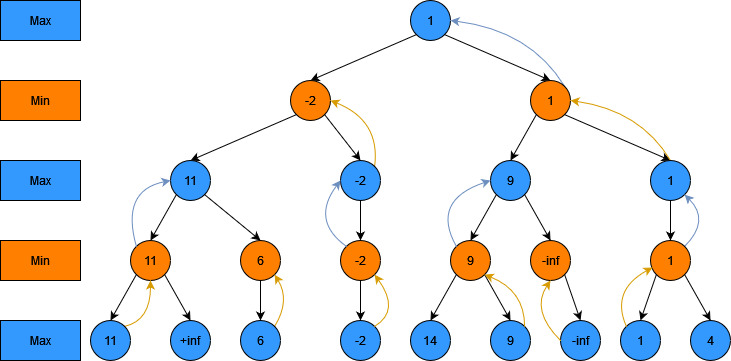
\includegraphics[width=0.4\textwidth]{root/MinMax.jpeg}
    \end{center}
    \caption{Ici, le joueur bleu cherche à maximiser ses gains avec une profondeur 4.}\label{fig:min_max}
\end{figure}


\subsubsection{Élagage alpha-bêta}
L'algorithme MinMax effectue une exploration complète de l'arbre de recherche jusqu'à un niveau donné. L'élagage alpha-bêta permet d'optimiser 
cet algorithme sans en modifier le résultat. Pour cela, il ne réalise qu'une exploration
partielle de l'arbre. En effet, on observe qu'il n'est pas utile d'explorer les sous-arbres qui conduisent à des valeurs
qui ne participeront pas au calcul de la valeur associée à la racine de l'arbre. Dit autrement, l'élagage alpha-bêta n'évalue pas des nœuds
dont on peut penser, si la fonction d'évaluation est à peu près correcte, que leur qualité sera inférieure à celle d'un nœud déjà évalué.

\begin{figure}[h]
    \begin{center}
        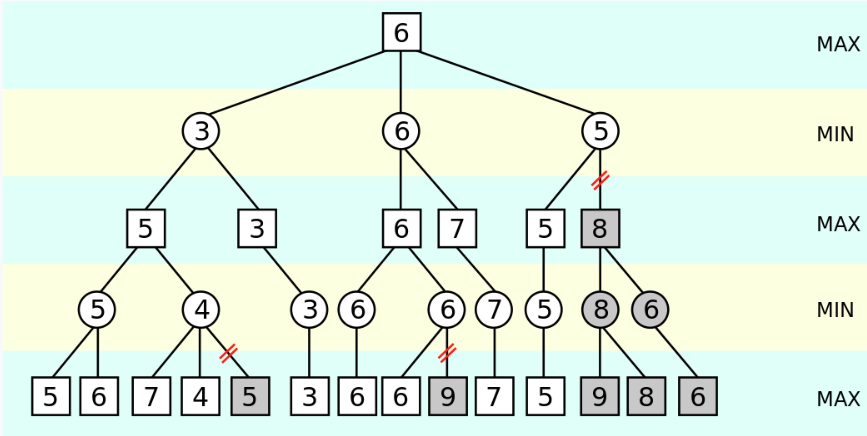
\includegraphics[width=0.5\textwidth]{root/minmax_alpha_beta.png}
    \end{center}
    \caption{MinMax avec élagage $\alpha$-$\beta$.}\label{fig:min_max_alpha_beta}
\end{figure}


Plusieurs coupures ont pu être réalisées. De gauche à droite :
\begin{enumerate}
    \item Le nœud MIN vient de mettre à jour sa valeur courante à 4. Celle-ci, qui ne peut que baisser, est déjà inférieure à $\alpha$=5, 
    la valeur actuelle du nœud MAX précédent. Celui-ci cherchant la plus grande valeur possible, ne la choisira donc de toute façon pas.
    \item Le nœud MIN vient de mettre à jour sa valeur courante à 6. Celle-ci, qui ne peut que baisser, est déjà égale à $\alpha$=6, la valeur 
    actuelle du nœud MAX précédent. Celui-ci cherchant une valeur supérieure, il ne mettra de toute façon pas à jour sa valeur que ce nœud 
    vaille 6 ou moins.
    \item Le nœud MIN vient de mettre à jour sa valeur courante à 5. Celle-ci, qui ne peut que baisser, est déjà inférieure à $\alpha$=6, la valeur 
    actuelle du nœud MAX précédent. Celui-ci cherchant la plus grande valeur possible, ne la choisira donc de toute façon pas.
\end{enumerate}

\subsubsection{Remarques:}
À l'aide de l'algorithme MinMax, il est possible de donner une preuve de l'existence d'une stratégie gagnante au jeu du Hex notamment. Nous détaillons
cette preuve en annexe.

\subsection{Autres algorithmes}
\subsubsection{Dijkstra et BFS}
Dans le projet lorsque un joueur gagne au Hex le chemin le plus court entre ses deux bords du plateau est mis en valeur
pour cela nous devions d'abord detecter qu'un joueur ait gagné. Pour cela nous avons implementé l'algorithme du parcours
en largeur (BFS) en interpretant le tableau dans lequel les coups des joueurs est sauvegradé comme une graphe.Le parcous en profondeur
va generer un graphe couvrant depuis un bord en ne passant que par des coups placés par un joueur, si le graphe generé attein le bord opposé
alors le joueur a gagné. Nous appellons cet algorithme a chaque fois qu'un coup est placé et celui ci est de complexité O(|V|+|E|).
Notons ici que nous appelons l'algo seulement sur l'arbre correspondant aux coups joué par un joueur, donc en pratique l'appel a cet algorithme
est tres rapide.

Ensuite nous voulions mettre en valeur le chemin le plus court qui relie les 2 bords du joueur qui a gagné. Pour cela,
nous avons utilisé l'algorithme de dijkstra un peu modifié en effet le BFS nous assure qu'un chemin existe mais ne nous aide pas vraiment
a trouver le plus court en effet il peut y avoir plusieurs points de departs (point sur le bord) et point d'arrivée (points sur le bord opposé)
Nous avons opté pour une solution naive, nous appellons l'algorithme plusieurs fois (une pour chaque point de depart possible)
puis nous comparons la taille des chemins trouvés. La complexité de dijkstra est a l'orgigine dans le pire des cas de O(|V|+|E|*log(|V|)) 
mais notre implementation est plus complexe elle a une complexité dans le pire des cas de O(n*(|V|+|E|*log(|V|))) ou n est la taille de notre plateau
a noter que ce cas arrive en pratique jamais et il n'est appelé qu'une fois a la fin de chaque partie. En pratique le chemin le plus court est trouvé
instantanement.

\begin{figure}[h]
    \begin{center}
        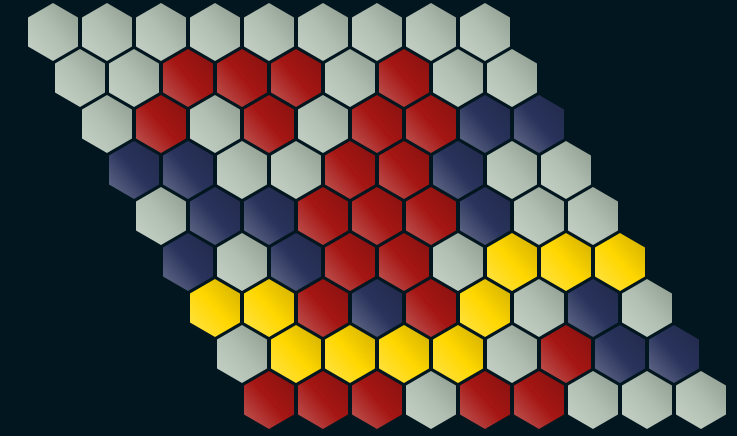
\includegraphics[width=0.5\textwidth]{root/chemin_gagnant.png}
    \end{center}
    \caption{Ici bleu a gagné et le chemin le plus court est trouvé}\label{fig:chemin_gagnant}
\end{figure}